%% Near-light photometric stereo for endoscopic bone measurement
%% Build:  pdflatex manuscript && pdflatex manuscript
\documentclass[journal,10pt]{IEEEtran}

\usepackage[T1]{fontenc}
\usepackage[utf8]{inputenc}
\usepackage{lmodern}
\usepackage{amsmath,amssymb,bm}
\usepackage{graphicx}
\usepackage{booktabs}
\usepackage{array}
\usepackage{multirow}
\usepackage{xcolor}
\usepackage[most]{tcolorbox}
\usepackage{microtype}
\usepackage{siunitx}
\sisetup{detect-all, range-phrase={--}, range-units=single,
         per-mode=symbol, group-digits=false}
\usepackage{url}
\usepackage[hidelinks]{hyperref}

\definecolor{todoRed}{HTML}{A11212}
\definecolor{todoBg}{HTML}{FDF3F3}
\definecolor{noteBg}{HTML}{F4F6F9}
\definecolor{noteBorder}{HTML}{5B6B7F}

%% Placeholder / not-yet-done block. Deliberately loud.
\newtcolorbox{todobox}[1]{
  breakable, enhanced, colback=todoBg, colframe=todoRed,
  boxrule=0.6pt, left=5pt, right=5pt, top=4pt, bottom=4pt,
  fonttitle=\bfseries\footnotesize, title={#1}, coltitle=white,
  colbacktitle=todoRed, sharp corners=downhill}

%% Neutral note block (open questions that are not placeholders)
\newtcolorbox{notebox}[1]{
  breakable, enhanced, colback=noteBg, colframe=noteBorder,
  boxrule=0.5pt, left=5pt, right=5pt, top=4pt, bottom=4pt,
  fonttitle=\bfseries\footnotesize, title={#1}, coltitle=white,
  colbacktitle=noteBorder, sharp corners=downhill}

\newcommand{\TODO}[1]{\textcolor{todoRed}{\textbf{[#1]}}}
\newcommand{\vecn}{\bm{n}}
\newcommand{\vecg}{\bm{g}}
\newcommand{\vecx}{\bm{x}}
\newcommand{\vecm}{\bm{m}}
\newcommand{\vecP}{\bm{P}}

\begin{document}

\title{Near-Light Photometric Stereo for Endoscopic Bone Surface Measurement:
Ring-LED Calibration, Offset--Scale Geometry, and Fiducial-Anchored
Registration to CT}

\author{\TODO{AUTHOR LIST}%
\thanks{Manuscript draft v0.3. Sections on endoscope-to-CT registration
(Sec.~\ref{sec:reg}, Sec.~\ref{sec:regresults}) are marked placeholders and are
not yet complete. All other reported values are reproduced from the committed
pipeline outputs and are traceable to a named file and column. Every derivation
in Sec.~\ref{sec:calibgeom}--\ref{sec:ledcalib} was independently re-derived and
numerically cross-checked, and the caveats reported throughout --- including the
scale conflict of Sec.~\ref{sec:scaleconflict} and the self-test limitations of
Sec.~\ref{sec:selftest} --- are outcomes of that audit.}%
\thanks{\TODO{AFFILIATIONS, CORRESPONDING AUTHOR, FUNDING}}}

\markboth{Draft v0.3 --- not for circulation}{Near-Light Photometric Stereo for
Endoscopic Bone Surface Measurement}

\maketitle

\begin{abstract}
\textbf{\textit{Background---}}Image-guided intervention on bone requires a
spatial correspondence between the intra-operative endoscopic view and a
pre-operative CT volume. Establishing that correspondence demands metric
three-dimensional surface information, which a monocular endoscope does not
natively provide. Photometric stereo is attractive because the emitters are
already integrated into the instrument tip, but its classical formulation
assumes distant, directional illumination --- an assumption that endoscopic
geometry violates severely.
\textbf{\textit{Purpose---}}To present a near-light photometric stereo pipeline
for a four-LED ring endoscope, comprising the ring geometry and its offset and
scale calibration, a calibrated point-source forward model, a perspective
log-depth solver, retroreflective fiducial localization, and fiducial-anchored
transfer into the CT frame; and to quantify, against CT ground truth, the error
incurred by the far-field approximation at this geometry.
\textbf{\textit{Methods---}}Four LEDs are mounted \SI{90}{\degree} apart on a
ring of measured radius \SI{12.08}{\milli\metre} about the lens and sequenced
individually by a microcontroller, giving four single-emitter exposures plus an
ambient frame per session at a measured \SI{30}{\milli\metre} working distance
over a \SI{37}{\milli\metre} field. The offset-to-working-distance ratio is
\num{0.40}, placing the rig unambiguously in the near field. We derive the
perspective log-depth relation used to integrate normals metrically, and
implement the LED calibration of Qu\'eau \textit{et al.} recovering per-emitter
position, principal direction, anisotropy and intensity. Five sessions of an
ex-vivo vertebral specimen were processed; one carries CT ground truth for three
fiducials, transferred into the camera frame by a P3P solution disambiguated
with a confirmed ordinal constraint.
\textbf{\textit{Results---}}Fiducial localization recovered 18 markers, 14
(\SI{78}{\percent}) confirmed independently under all four illumination
directions. Against CT, the far-field depth estimate proved
\emph{anti-correlated} with true lens-to-marker distance ($r=-0.923$), reversing
the near-to-far ordering of all three CT-known fiducials; least-squares affine
rescaling onto the CT control points returned a \emph{negative} slope and left a
\SI{4.36}{\milli\metre} RMS residual over a \SI{20.7}{\milli\metre} true span.
The near-light solver and its calibration pass synthetic self-tests to
\SI{0.00}{\milli\metre} in emitter position and \SI{0.090}{\degree} in principal
direction.
\textbf{\textit{Conclusions---}}Fiducial localization and CT/P3P distances are
reliable and serve as registration inputs. The far-field depth channel is not
merely imprecise but sign-inverted at this geometry, and must not propagate into
a registration result; the calibrated near-light formulation is the corrective
path. \TODO{REGISTRATION RESULT PENDING}
\end{abstract}

\begin{IEEEkeywords}
Photometric stereo, near-field illumination, endoscopy, LED calibration,
retroreflective fiducials, image registration, surgical navigation.
\end{IEEEkeywords}

\section{Introduction}
\IEEEPARstart{R}{egistering} an endoscopic view to a pre-operative CT volume is
the enabling step for image-guided intervention on bone. The problem is well
posed only when the endoscopic side of the correspondence carries
three-dimensional, metrically-scaled information. A monocular endoscope does not
supply this directly, so it must be recovered --- from motion, from structured
illumination, or, as here, from shading.

Photometric stereo recovers surface orientation from the way brightness varies
as the illumination direction changes. It suits endoscopy because the light
sources are already present at the instrument tip: no additional hardware enters
the surgical field, and no relative motion between camera and specimen is
required. The classical formulation, however, assumes \emph{far-field}
illumination --- that each source is distant enough for its direction to be
constant across the field of view and for its intensity not to fall off within
the scene.

Endoscopic rigs violate both assumptions comprehensively. On the instrument
described here the emitters sit \SI{12.08}{\milli\metre} off the optical axis at
a \SI{30}{\milli\metre} working distance, a ratio of \num{0.40}. The direction
to a given emitter therefore sweeps by tens of degrees across the
\SI{37}{\milli\metre} field, and inverse-square falloff is a first-order effect
rather than a correction term. The correct treatment is \emph{near-light}
photometric stereo: a calibrated point-source forward model with per-pixel light
vectors, solved under perspective rather than orthographic projection.

This paper presents that pipeline end to end, and reports as its principal
empirical contribution a CT-validated measurement of what the far-field
shortcut costs at this geometry. The answer is worse than a scale error: the
recovered depth is \emph{anti-correlated} with truth, reversing the depth
ordering of the fiducials outright. We regard this as the more useful
contribution, because the far-field shortcut is widely taken in endoscopic
shading work and the \emph{sign} of the resulting error appears not to have been
measured against ground truth in this configuration.

\subsection{Contributions}
\begin{enumerate}
\item A complete near-light photometric stereo pipeline for a ring-LED
endoscope, with the ring geometry, its offset and scale calibration, and the
resulting camera model stated as measured quantities with explicit provenance
(Sec.~\ref{sec:system}--\ref{sec:calibgeom}).
\item A self-contained derivation of the perspective log-depth integration used
to recover metric depth from calibrated near-light normals
(Sec.~\ref{sec:logdepth}).
\item An implementation and synthetic validation of per-emitter photometric
calibration --- position, principal direction, anisotropy, intensity ---
following Qu\'eau \textit{et al.}~\cite{queau2018led} (Sec.~\ref{sec:ledcalib}).
\item A retroreflective fiducial detector exploiting the glass-bead sparkle
signature, with a cross-frame confirmation statistic
(Sec.~\ref{sec:fiducials}).
\item A quantified, CT-validated demonstration that far-field photometric stereo
inverts depth ordering at endoscopic near-light geometry
(Sec.~\ref{sec:inversion}).
\item \TODO{REGISTRATION CONTRIBUTION --- PENDING, Sec.~\ref{sec:reg}}
\end{enumerate}

\section{System Design}\label{sec:system}

\subsection{Optical head and LED ring}
The instrument is a monocular endoscope with four LEDs mounted on a ring
concentric with the lens, spaced \SI{90}{\degree} apart in azimuth
(Fig.~\ref{fig:rig}a). Writing $\mathrm{L}i$ for the emitter at azimuth
$\alpha_i$, the layout is
\begin{equation}
\alpha_1 = \SI{0}{\degree},\quad
\alpha_2 = \SI{90}{\degree},\quad
\alpha_3 = \SI{180}{\degree},\quad
\alpha_4 = \SI{270}{\degree},
\end{equation}
all at the same measured ring radius $r_\mathrm{LED}$. In the camera frame
(Sec.~\ref{sec:frame}) the emitter centres lie in the lens plane $Z=0$ at
\begin{equation}
\vecx_s^{(i)} = \bigl(r_\mathrm{LED}\cos\alpha_i,\;
-r_\mathrm{LED}\sin\alpha_i,\; 0\bigr)^{\!\top},
\label{eq:ledpos}
\end{equation}
the minus sign on the second component arising because azimuth is measured
counter-clockwise from $+X$ while $Y$ points \emph{down}.

The four emitters are nominally identical. Equal emitter power is not assumed by
the near-light solver, which takes per-emitter intensity from calibration
(Sec.~\ref{sec:ledcalib}); where emitters are genuinely identical the common
factor folds into albedo and cancels in the normalization
$\vecn = \vecg/\lVert\vecg\rVert$.

\subsection{Illumination sequencing}
The ring is driven by an Arduino Pro microcontroller, which switches exactly one
emitter at a time and holds the remaining three dark, so that each exposure
isolates a single known illumination direction. A fifth exposure is captured
with all emitters off to record the ambient component. Because the sequence is
electronically controlled while the camera and specimen remain stationary, the
five frames of a session are pixel-registered by construction --- a property the
fiducial consolidation of Sec.~\ref{sec:consolidation} exploits directly.

\begin{todobox}{Hardware details to record}
The specific Arduino Pro variant, the LED part number, the drive current, and
the exposure/frame timing are not yet recorded in the repository. The LED
datasheet half-power angle $\theta_{1/2}$ is required by the anisotropy step of
Sec.~\ref{sec:aniso} and must be obtained from the part datasheet. See
Appendix~\ref{app:open}, item~C1.
\end{todobox}

\subsection{Coordinate conventions}\label{sec:frame}
All quantities use a single right-handed camera frame: $X$ to the right, $Y$
downward, $Z$ from the lens into the scene, origin at the optical centre, units
of millimetres. Azimuth is measured counter-clockwise from $+X$ in the lens
plane. Depth $Z$ is positive into the scene, so a point farther from the lens
has larger $Z$. Outward-facing surface normals --- those pointing back toward
the camera --- therefore have $n_3 < 0$, a convention used throughout
Sec.~\ref{sec:nlps} and enforced explicitly in the solver.

\subsection{Capture protocol}
Each session ("shot") is a directory of five exposures of a static scene:
\texttt{led1.png}--\texttt{led4.png}, one per emitter, and \texttt{dark.png}
with all emitters off. A session is admitted to processing only if all four
single-emitter frames are present. Table~\ref{tab:invariants} states the
acquisition contract explicitly, since every downstream stage depends on it.

\begin{table}[t]
\centering
\caption{Acquisition invariants within one capture session.}
\label{tab:invariants}
\footnotesize
\begin{tabular}{@{}p{0.28\columnwidth}p{0.28\columnwidth}p{0.34\columnwidth}@{}}
\toprule
\textbf{Quantity} & \textbf{Status} & \textbf{Consequence} \\
\midrule
Camera pose & held constant & frames pixel-registered by construction \\
Specimen pose & held constant & a fiducial occupies the same pixel in every frame \\
Illumination direction & varied (4 emitters) & the photometric signal \\
Ambient light & measured once & subtracted per frame \\
Exposure & nominally fixed, normalized in software & Sec.~\ref{sec:exposure} \\
\bottomrule
\end{tabular}
\end{table}

\begin{figure*}[t]
\centering
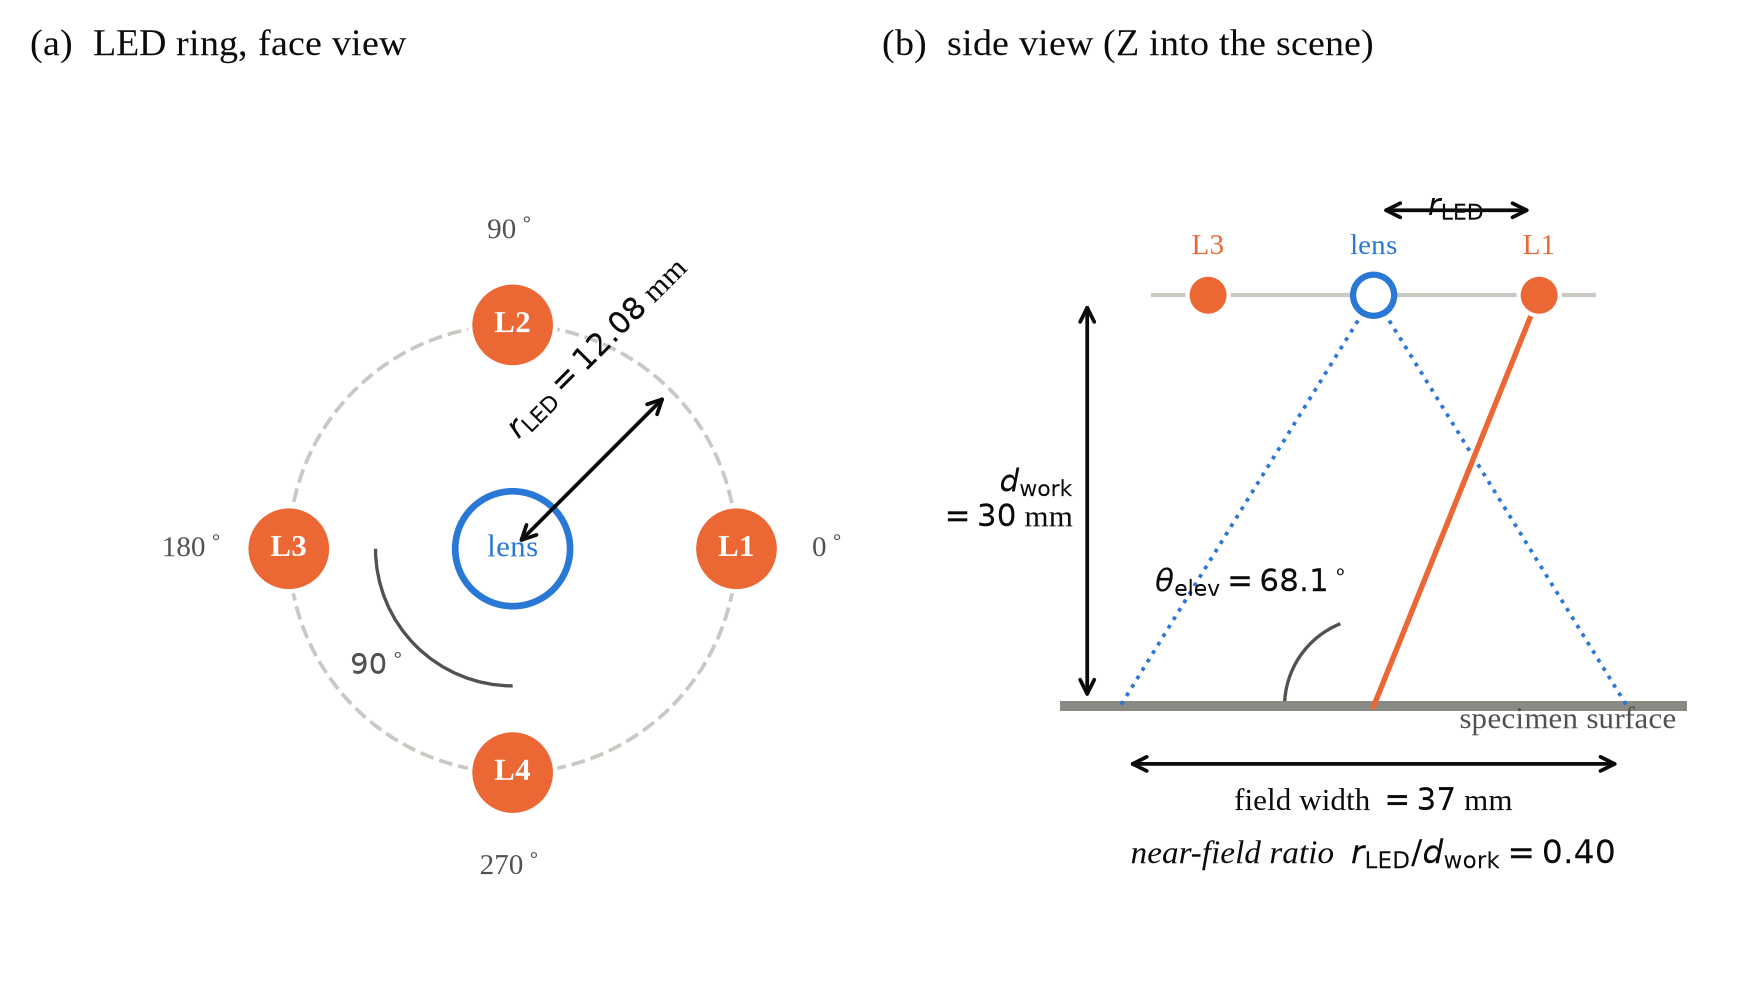
\includegraphics[width=0.86\textwidth]{fig1_rig.png}
\caption{System geometry. (a) Face view of the LED ring: four emitters
\SI{90}{\degree} apart at the measured radius
$r_\mathrm{LED}=\SI{12.08}{\milli\metre}$ about the lens. (b) Side view showing
the measured working distance $d_\mathrm{work}=\SI{30}{\milli\metre}$, the
\SI{37}{\milli\metre} field width, and the resulting illumination elevation
$\theta_\mathrm{elev}=\SI{68.1}{\degree}$ at the on-axis surface point. The
offset-to-working-distance ratio of \num{0.40} is what places this rig in the
near field and makes the far-field approximation inadmissible
(Sec.~\ref{sec:whyfar}). All dimensions are measured values.}
\label{fig:rig}
\end{figure*}

\section{Geometric Calibration: Offset and Scale}\label{sec:calibgeom}

Two measured lengths govern the entire pipeline: the ring \emph{offset}
$r_\mathrm{LED}$, which sets the illumination geometry and the near-field
regime; and the field \emph{scale}, which converts pixels to millimetres and
fixes the camera's focal length. Table~\ref{tab:geom} lists every geometric
parameter with its provenance --- a distinction that matters here because the
measured and calibration-derived values disagree
(Sec.~\ref{sec:ambiguity}).

\begin{table}[t]
\centering
\caption{Rig and imaging parameters. Frame: $X$ right, $Y$ down, $Z$ into the
scene, origin at the optical centre.}
\label{tab:geom}
\footnotesize
\begin{tabular}{@{}ll l p{0.24\columnwidth}@{}}
\toprule
\textbf{Symbol} & \textbf{Value} & \textbf{Provenance} & \textbf{Role} \\
\midrule
$r_\mathrm{LED}$ & \SI{12.08}{\milli\metre} & measured & ring offset \\
field width      & \SI{37.0}{\milli\metre}  & measured & scale \\
$d_\mathrm{work}$& \SI{30.0}{\milli\metre}  & measured & working distance \\
$\theta_\mathrm{elev}$ & \SI{68.1}{\degree} & derived  & elevation \\
$s$              & \num{0.05781}\,mm/px     & derived  & in-plane scale \\
$f_x$            & \num{519}\,px            & derived  & focal length \\
$f_x$ (chkbd.)   & \num{794}\,px            & calibrated & \textbf{conflicts} (Sec.~\ref{sec:ambiguity}) \\
$W$              & \num{640}\,px            & config.  & working resolution \\
$\theta_{1/2}$   & \TODO{TBD}               & datasheet & emitter anisotropy \\
\bottomrule
\end{tabular}
\end{table}

\subsection{The offset and the illumination elevation}
The elevation of an emitter above the surface plane, evaluated at the surface
point on the optical axis, follows from the right triangle formed by the ring
offset and the working distance:
\begin{equation}
\theta_\mathrm{elev}
= \arctan\!\left(\frac{d_\mathrm{work}}{r_\mathrm{LED}}\right)
= \arctan\!\left(\frac{30.0}{12.08}\right) = \SI{68.1}{\degree}.
\label{eq:elev}
\end{equation}
This value is \emph{derived} from the two measured lengths rather than assumed.
It is, however, the \emph{on-axis} elevation, and it is the single constant the
far-field baseline applies to every pixel. Across the \SI{37}{\milli\metre} field
along the emitter's axis the true elevation ranges from \SI{44.5}{\degree}
through \SI{90}{\degree} to \SI{77.9}{\degree}; evaluated at the three CT-known
fiducial positions in the recovered camera frame it takes the values
\SI{74.9}{\degree}, \SI{83.5}{\degree} and \SI{57.9}{\degree}, against the
constant \SI{68.1}{\degree} actually used. That spread is the far-field
approximation made visible, and it is precisely the point of
Sec.~\ref{sec:whyfar}.

\subsection{The scale and the camera model}
Images are undistorted and resized so the long edge is $W=\num{640}$\,px; a
pinhole model with
\begin{equation}
K = \begin{bmatrix} f_x & 0 & c_x \\ 0 & f_y & c_y \\ 0 & 0 & 1 \end{bmatrix}
\end{equation}
is used thereafter, with the principal point at the image centre. The in-plane
scale at the working distance is
\begin{equation}
s = \frac{\text{field width}}{W} = \frac{37.0}{640}
  = \SI{0.05781}{\milli\metre\per pixel}.
\label{eq:scale}
\end{equation}
Rather than adopt the checkerboard focal length, the pipeline derives $f_x$ from
the same two measured lengths. For a pinhole camera imaging a field of metric
width $\Omega$ at distance $d$ onto $W$ pixels, similar triangles give
$\Omega/d = W/f_x$, hence
\begin{equation}
f_x = \frac{W\, d_\mathrm{work}}{\Omega} = \frac{640 \times 30.0}{37.0}
    = \SI{519}{pixel}.
\label{eq:fx}
\end{equation}
The vertical focal length follows from the same distance and the field height
$\tfrac{3}{4}\Omega$, which encodes a \num{4}:\num{3}-shaped physical field
irrespective of the frame's aspect ratio; at the \num{4}:\num{3} working
resolution actually used ($640\times480$) it correctly yields $f_y = f_x$. Note
that Eqs.~\eqref{eq:scale} and~\eqref{eq:fx} are consistent by construction:
$d_\mathrm{work}/f_x = F/W = s$ identically.

Two caveats on the scale must be stated. First, $s$ is the scale \emph{at the
working distance only}: the true in-plane scale is $Z/f_x$ and therefore varies
with depth, so applying the constant $s$ across a depth map is itself a
small-relief approximation. Second, the principal point is set to the image
centre, whereas the calibration --- transported to the undistorted working frame
--- places it near $(324.1,\,225.5)$, a vertical discrepancy of
\SI{14.5}{pixel}. The docstring's stated intent is that only the absolute focal
length be replaced; in fact $c_x, c_y$ are silently replaced too. The effect on
the reported CT distances is \SIrange{0.1}{0.7}{\milli\metre} --- small, but a
straightforward correctness fix.

\subsection{The focal-length ambiguity}\label{sec:ambiguity}
The checkerboard calibration returns $f_x = \SI{1588}{pixel}$ at native
resolution, i.e. \SI{794}{pixel} at the \num{640}\,px working width --- a factor
of \num{1.53} above Eq.~\eqref{eq:fx}. Equivalently, the calibrated focal length
implies a \SI{45.9}{\milli\metre} working distance for a \SI{37}{\milli\metre}
field where \SI{30}{\milli\metre} was measured, and a field of view near
\SI{44}{\degree} where the measured pair imply roughly \SI{63}{\degree}.

We resolve this in favour of the bench measurements, on the grounds that the two
measurements are mutually consistent while the checkerboard result contradicts
both. This is an arbitration, not a resolution. Every \emph{absolute} distance
in this paper therefore carries an unresolved ${\sim}1.5\times$ scale
uncertainty; relative comparisons within a session are unaffected, since the
ambiguity is a single multiplicative factor.

\begin{todobox}{Calibration residuals not recorded}
The checkerboard reprojection error, the number and spread of calibration poses,
and the distortion coefficients are not currently recorded. A calibration
reported without its residuals cannot be assessed, and the residual may itself
explain the \num{1.53}$\times$ discrepancy. The ambiguity is settled definitively
by imaging an object of known size at a known distance. See
Appendix~\ref{app:open}, item~C2.
\end{todobox}

\section{Near-Light Photometric Stereo}\label{sec:nlps}

\subsection{Why the far-field model is inadmissible here}\label{sec:whyfar}
Far-field photometric stereo requires that the direction to each source be
constant over the field and that intensity falloff within the scene be
negligible. The governing dimensionless quantity is the ratio of source offset
to working distance,
\begin{equation}
\eta = \frac{r_\mathrm{LED}}{d_\mathrm{work}} = \frac{12.08}{30.0} = 0.40 ,
\end{equation}
which is order unity rather than small. Two consequences follow directly. First,
the direction from a surface point to a given emitter varies across the
\SI{37}{\milli\metre} field by tens of degrees, so no single constant light
vector describes the emitter. Second, the emitter-to-surface distance varies by
well over \SI{10}{\percent} across the same span, so the $1/r^2$ term cannot be
absorbed into a constant.

Neglecting both produces a smooth, low-spatial-frequency brightness bias that
the normal-recovery step misinterprets as surface tilt. Integration then
accumulates that spurious tilt into a large-scale curvature which dominates the
genuine relief. Section~\ref{sec:inversion} measures the result against CT: at
this geometry the error is not a scale factor but a sign inversion.

\subsection{Near-light irradiance model}\label{sec:forward}
We adopt the LED model of Qu\'eau \textit{et al.}~\cite{queau2018led}. For
emitter $i$ with position $\vecx_s^{(i)}$, unit principal direction
$\vecn_s^{(i)}$, anisotropy exponent $\mu_i$ and intensity $\Psi_i$, the
irradiance at a surface point $\vecx$ with unit normal $\vecn$ and albedo $\rho$
is
\begin{equation}
I^{(i)} = \Psi_i\,\rho\,
\underbrace{\left[\frac{\vecn_s^{(i)}\!\cdot(\vecx-\vecx_s^{(i)})}
                       {\lVert \vecx-\vecx_s^{(i)}\rVert}\right]^{\mu_i}}
          _{\cos^{\mu_i}\theta,\ \text{angular profile}}
\underbrace{\frac{\bigl\{(\vecx_s^{(i)}-\vecx)\cdot\vecn\bigr\}_+}
                 {\lVert\vecx_s^{(i)}-\vecx\rVert^{3}}}
          _{\text{Lambert} \times 1/r^2} ,
\label{eq:forward}
\end{equation}
where $\{\cdot\}_+$ denotes clamping at zero (self-shadowing) and $\theta$ is
the emission angle off the emitter's principal axis. The cubic power in the
denominator is not a typographical accident: one power normalizes the
un-normalized dot product in the numerator into a cosine, leaving $1/r^2$
attenuation.

It is convenient to gather the geometry into a per-pixel \emph{effective light
vector}. Writing $\bm{d} = \vecx_s - \vecx$, $r = \lVert\bm{d}\rVert$ and
$\bm{\omega} = \bm{d}/r$, Eq.~\eqref{eq:forward} becomes
$I^{(i)} = \rho\,\bm{v}^{(i)}\!\cdot\vecn$ with
\begin{equation}
\bm{v}^{(i)}(\vecx) = \Psi_i\,
\frac{\bigl(\max(-\bm{\omega}\cdot\vecn_s^{(i)},\,0)\bigr)^{\mu_i}}{r^{2}}\,
\bm{\omega} .
\label{eq:lightvec}
\end{equation}
Every factor in Eq.~\eqref{eq:lightvec} --- $\vecx_s$, $\vecn_s$, $\mu$, $\Psi$
--- comes from calibration (Sec.~\ref{sec:ledcalib}); none is assumed from rig
symmetry. This is the essential difference from the far-field baseline, in which
$\bm{v}^{(i)}$ is a single constant unit vector for the whole image.

\subsection{Specular-free channel}
Bone is wet and glossy, and the retroreflective fiducials are strongly
non-Lambertian, so the Lambertian model of Eq.~\eqref{eq:forward} cannot be
applied to raw intensity. We use a dichromatic separation: under the dichromatic
reflection model the surface-reflection (specular) component carries the
illuminant's spectrum while the body-reflection component carries the surface
spectrum. For an illuminant whose linear red and blue responses are equal, the
difference
\begin{equation}
I_\mathrm{body} = \max\bigl(I_R^{\mathrm{lin}} - I_B^{\mathrm{lin}},\; 0\bigr)
\end{equation}
cancels the specular term and retains a signal proportional to body reflection.
Writing $I_c = m_d B_c + m_s E_c$ for channel $c$, with $m_d, m_s$ the geometric
body and surface factors and $B_c, E_c$ the corresponding spectral integrals,
\begin{equation}
I_R - I_B = m_d(B_R - B_B) + m_s(E_R - E_B),
\end{equation}
so the specular term vanishes \emph{iff} $E_R = E_B$. The residual
$(B_R-B_B)$ is a per-pixel material constant identical across the four frames,
so it folds into the pseudo-albedo and cancels in
$\vecn = \vecg/\lVert\vecg\rVert$.

\begin{notebox}{The precise assumption, and its sensitivity}
The requirement is not that the emitter be ``white'' colorimetrically, but that
it produce \emph{equal linear $R$ and $B$ responses in this camera}, after
whatever white balance and colour matrix the pipeline applies. Phosphor-converted
white LEDs have a strongly non-flat spectrum, so this holds by construction only
if the camera is balanced on a neutral target \emph{under these emitters}.
The failure is not graceful: a \SI{5}{\percent} $R/B$ imbalance leaks
${\sim}\SI{18}{\percent}$ of the specular signal into the body channel, and that
leak has exactly the specular lobe's geometry --- concentrated where it does most
damage. The measured $E_R/E_B$ of the rig on a neutral target should be reported.

A second, smaller effect: clamping the difference at zero is a nonlinear
operation that rectifies noise where the signal is near zero, i.e. in shadow and
background. In simulation this biases shadowed pixels ${\sim}\SI{25}{\percent}$
high while leaving well-lit pixels unbiased --- and shadowed pixels are exactly
where a $K$-light solve is already most fragile.
\end{notebox}

\subsection{Exposure normalization}\label{sec:exposure}
Camera gain is a single global multiplier that scales all channels equally, so
it is estimated from linear luminance --- which stays positive in shadow --- over
the well-lit region, and the body-reflection frame is divided by that scalar.

This detail is worth reporting because the obvious alternative is wrong.
Normalizing each frame by the median of its \emph{own} specular-free channel
fails: that channel is near zero over dark background and single-emitter shadow,
so its median can collapse toward zero, and dividing by it injects a large
spurious per-emitter gain. A factor of ${\sim}250\times$ was observed from this
mechanism before the estimator was moved onto luminance.

\subsection{Per-pixel normal recovery}
For $K$ emitters the model is linear in the albedo-scaled normal
$\vecg = \rho\,\vecn$. Stacking the per-pixel effective light vectors of
Eq.~\eqref{eq:lightvec} as rows of $M \in \mathbb{R}^{K\times3}$ and the
observed body intensities as $\bm{I}\in\mathbb{R}^{K}$,
\begin{equation}
M\vecg = \bm{I},
\qquad
\vecg = (M^{\!\top}\!M + \epsilon \mathbb{I})^{-1} M^{\!\top}\bm{I},
\label{eq:normalsolve}
\end{equation}
with a small $\epsilon$ for conditioning. The normal equations are used so the
same code path serves $K=3$ (exact) and $K=4$ (least squares, the ring rig here)
without special-casing.

Two properties of this system deserve statement rather than assumption. The
emitters sit only \SI{21.9}{\degree} off the optical axis at
\SI{12.08}{\milli\metre} and \SI{30}{\milli\metre}, so the configuration is
inherently narrow-baseline: $\operatorname{cond}(M)\approx5.4$ on axis, and
forming the normal equations squares it to
$\operatorname{cond}(M^{\!\top}\!M)\approx28.8$, rising to \num{49.7} off axis.
And the regularizer is \emph{absolute}: at millimetre scale
$\lVert\bm{v}\rVert\sim\Psi/r^2$ is small enough that a fixed
$\epsilon=10^{-9}$ amounts to \SIrange{0.5}{2.9}{\percent} of the smallest
eigenvalue, inducing a systematic, spatially varying normal tilt of
\SIrange{0.04}{0.30}{\degree} that grows with depth and off-axis distance. A
relative form $\epsilon = \lambda\operatorname{tr}(M^{\!\top}\!M)/3$ would be
scale-invariant; as written the term is physically scaled, not merely numerical,
and would silently change meaning if the code were switched to metres. Albedo
and unit normal follow as
\begin{equation}
\rho = \lVert\vecg\rVert, \qquad \vecn = \vecg/\rho ,
\end{equation}
and the sign is fixed by the outward convention of Sec.~\ref{sec:frame}: any
normal with $n_3 > 0$ is negated, so that all normals face the camera.

Crucially, $M$ varies from pixel to pixel because $\bm{v}^{(i)}$ depends on the
surface point $\vecx$ --- which is what the solver is trying to find. This
circularity is resolved by iteration (Sec.~\ref{sec:iterate}).

\subsection{Perspective log-depth integration}\label{sec:logdepth}
Given normals, depth must be recovered by integration. Under \emph{orthographic}
projection one integrates $\partial z/\partial u = n_1/n_3$ directly; that is
systematically wrong here, because the relief is a substantial fraction of the
working distance and the metric footprint of a pixel therefore changes across
the surface. The correct treatment is perspective.

Let $x_t = (u-c_x)/f_x$ and $y_t = (v-c_y)/f_y$, so that a surface point imaged
at pixel $(u,v)$ with depth $Z(u,v)$ is
\begin{equation}
\vecP(u,v) = Z(u,v)\,\bigl(x_t,\; y_t,\; 1\bigr)^{\!\top}.
\end{equation}
Differentiating along the image axes, and using
$\partial x_t/\partial u = 1/f_x$ and $\partial y_t/\partial u = 0$,
\begin{align}
\frac{\partial \vecP}{\partial u}
&= \frac{\partial Z}{\partial u}\,(x_t, y_t, 1)^{\!\top}
 + Z\left(\tfrac{1}{f_x},\,0,\,0\right)^{\!\top}, \\
\frac{\partial \vecP}{\partial v}
&= \frac{\partial Z}{\partial v}\,(x_t, y_t, 1)^{\!\top}
 + Z\left(0,\,\tfrac{1}{f_y},\,0\right)^{\!\top}.
\end{align}
The normal is orthogonal to both surface tangents,
$\vecn\cdot\partial_u\vecP = \vecn\cdot\partial_v\vecP = 0$. Substituting and
writing
\begin{equation}
D \;\equiv\; \vecn\cdot(x_t, y_t, 1)^{\!\top} \;=\; n_1 x_t + n_2 y_t + n_3 ,
\label{eq:Ddef}
\end{equation}
the first condition gives $D\,\partial_u Z + Z n_1/f_x = 0$, hence
\begin{equation}
\frac{1}{Z}\frac{\partial Z}{\partial u} = -\frac{n_1}{f_x D},
\qquad
\frac{1}{Z}\frac{\partial Z}{\partial v} = -\frac{n_2}{f_y D},
\end{equation}
and since $\partial(\ln Z)/\partial u = Z^{-1}\partial Z/\partial u$,
\begin{equation}
\boxed{\;
\frac{\partial \ln Z}{\partial u} = -\frac{n_1}{f_x D},
\qquad
\frac{\partial \ln Z}{\partial v} = -\frac{n_2}{f_y D}. \;}
\label{eq:logdepth}
\end{equation}
The problem is therefore linear in $\ln Z$, not in $Z$. The two gradient fields
of Eq.~\eqref{eq:logdepth} are integrated by an FFT Poisson solve enforcing
integrability, and the result is exponentiated.

Two implementation points matter. First, $D$ is clamped away from zero and held
negative ($D \le -0.10$), consistent with the outward convention $n_3<0$; this
bounds the gradient where the surface turns away from the camera. Second,
integration determines $\ln Z$ only up to an additive constant, so $Z$ is
determined only up to one global multiplicative scale. That scale is fixed by
anchoring the median depth over the specimen mask to the measured working
distance:
\begin{equation}
Z = d_\mathrm{work}\,
\exp\!\bigl(\ln Z' - \operatorname{median}_{\mathcal{M}} \ln Z'\bigr),
\label{eq:anchor}
\end{equation}
where $\ln Z'$ is the integrated field and $\mathcal{M}$ the specimen mask.
Because $\exp$ is strictly monotonic it maps the middle order statistic to the
middle order statistic, so Eq.~\eqref{eq:anchor} sets the median of $Z$ over
$\mathcal{M}$ to exactly $d_\mathrm{work}$ for an odd number of mask pixels. For
an even count the usual tie-break averages the two central values, and
$\exp$ of their arithmetic mean is their geometric mean, differing by a factor
$\cosh\!\bigl((b-a)/2\bigr)$; for adjacent order statistics of ${\sim}10^5$
pixels this is a relative discrepancy below $10^{-12}$ and is negligible.

Two honest qualifications belong with this step. First, integration recovers
$\ln Z$ exactly only when $(p,q)$ is curl-free; with noisy normals it is not, and
the FFT solver returns the least-squares integrable approximation rather than the
field itself. Second, because the scale is re-anchored to $d_\mathrm{work}$ on
every sweep, the near-light model buys correct \emph{perspective foreshortening},
not absolute depth --- per-pixel albedo is unknown, so albedo and $r$ trade off
and absolute scale is imposed rather than solved.

\subsection{Fixed-point iteration}\label{sec:iterate}
Because the light vectors depend on the unknown geometry, the solver alternates:
\begin{enumerate}
\item initialize $Z$ to the constant working distance;
\item back-project to points $\vecP = Z\,(x_t,y_t,1)^\top$;
\item evaluate per-pixel light vectors, Eq.~\eqref{eq:lightvec};
\item solve for normals, Eq.~\eqref{eq:normalsolve};
\item integrate to depth, Eqs.~\eqref{eq:logdepth}--\eqref{eq:anchor};
\item repeat from step~2.
\end{enumerate}
Two iterations are used, and the choice is justified by a convergence sweep on
the synthetic scene rather than asserted. The alternation reaches a stable fixed
point within three to four sweeps: median normal error and recovered relief are
unchanged to four significant figures from sweep~4 through sweep~30, at two noise
levels. The first sweep, which evaluates the light vectors on a flat plane at the
working distance, systematically \emph{over-estimates} relief --- \SI{114.9}{
\percent} of truth --- because the $1/r^2$ falloff is evaluated at the wrong
depth. One refinement corrects this to \SI{99.6}{\percent}
(Table~\ref{tab:converge}). Two sweeps therefore sit within \SI{0.11}{\degree}
median normal error and \SI{0.8}{\percent} relief of the converged solution at
half the cost.

\begin{table}[t]
\centering
\caption{Convergence of the geometry--normals alternation on the synthetic
scene. The solution is a stable fixed point from sweep 4 onward, not a
degrading sequence.}
\label{tab:converge}
\footnotesize
\begin{tabular}{@{}rccc@{}}
\toprule
\textbf{Sweeps} & \textbf{median normal err.} & \textbf{relief ratio} &
\textbf{median depth err.} \\
\midrule
1  & \SI{2.628}{\degree} & 1.1486 & \SI{0.268}{\milli\metre} \\
2  & \SI{3.966}{\degree} & 0.9963 & \SI{0.308}{\milli\metre} \\
3  & \SI{3.855}{\degree} & 1.0044 & \SI{0.306}{\milli\metre} \\
4  & \SI{3.853}{\degree} & 1.0044 & \SI{0.306}{\milli\metre} \\
10 & \SI{3.854}{\degree} & 1.0044 & \SI{0.306}{\milli\metre} \\
30 & \SI{3.854}{\degree} & 1.0044 & \SI{0.306}{\milli\metre} \\
\bottomrule
\end{tabular}
\end{table}

\begin{notebox}{Wording to correct in the implementation}
The solver's docstring describes the loop as alternating ``until stable'' while
the code in fact runs a fixed count with no stability test, and attributes the
choice of two to a degradation at higher counts. The sweep above does not
reproduce any such degradation. Either add an explicit convergence criterion or
describe the constant as the cost/accuracy tradeoff it is; the current comment
would not survive a reviewer re-running the self-test.
\end{notebox}

\section{Photometric Calibration of the LED Ring}\label{sec:ledcalib}
The forward model of Eq.~\eqref{eq:forward} introduces four parameters per
emitter. Each has its own calibration procedure; none is assumed from ring
symmetry.

\subsection{Anisotropy from the datasheet}\label{sec:aniso}
The imperfect-Lambertian emitter profile is $\Phi(\theta)=\Phi_0\cos^\mu\theta$.
The datasheet half-power angle $\theta_{1/2}$ is where relative intensity falls
to one half, so $\cos^\mu\theta_{1/2} = \tfrac{1}{2}$ and
\begin{equation}
\mu = \frac{-\ln 2}{\ln\cos\theta_{1/2}} .
\label{eq:mu}
\end{equation}
A source with $\theta_{1/2}=\SI{60}{\degree}$ gives $\mu=1$ exactly --- a truly
Lambertian emitter --- and $\theta_{1/2}=\SI{45}{\degree}$ gives $\mu=2$; a
narrower beam gives larger $\mu$, with $\mathrm{d}\mu/\mathrm{d}\theta_{1/2}<0$
throughout $(0,\SI{90}{\degree})$.

\begin{notebox}{Datasheet convention --- a live trap}
Eq.~\eqref{eq:mu} takes the \emph{half}-angle $\theta_{1/2}$, but LED datasheets
almost universally quote the \emph{full} included viewing angle
$2\theta_{1/2}$: a part advertised as ``\SI{120}{\degree} viewing angle'' has
$\theta_{1/2}=\SI{60}{\degree}$ and hence $\mu=1$. Feeding the datasheet number
directly into Eq.~\eqref{eq:mu} silently yields $\mu=4.82$ instead of \num{2.00}
for a \SI{60}{\degree}-quoted part. The convention must be stated explicitly
alongside the recorded value.
\end{notebox}

\subsection{Emitter position by mirror-sphere triangulation}
A specular sphere of known radius $R$ is imaged in several poses. For each pose,
the sphere centre is recovered from its silhouette: the camera rays grazing the
sphere form a right circular cone about the direction to the centre, so the
boundary ray directions lie on a common plane $\bm{a}\cdot\bm{d}=\cos\beta$. The
axis $\bm{a}$ is estimated as the least-variance eigenvector of the boundary
directions, and the tangent-line geometry
\begin{equation}
\sin\beta = \frac{R}{\lVert \bm{C}\rVert}
\quad\Longrightarrow\quad
\bm{C} = \frac{R}{\sin\beta}\,\bm{a}
\end{equation}
fixes the range.

It is worth stating that $\cos\beta$ is estimated \emph{exactly}, not
approximately, and that the obvious alternative fails badly. Every boundary
direction satisfies $\bm{a}\cdot\bm{d}_k=\cos\beta$ individually, so by linearity
$\bm{a}\cdot\bar{\bm{d}} = \tfrac{1}{K}\sum_k \bm{a}\cdot\bm{d}_k = \cos\beta$
for \emph{any} sampling of the boundary --- uniform, clustered, or a short arc.
The mean direction $\bar{\bm{d}}$ is however \emph{not} a unit vector: for
uniform sampling $\bar{\bm{d}} = \cos\beta\,\bm{a}$, so normalizing it first and
taking $\arccos(\bm{a}\cdot\hat{\bar{\bm{d}}})$ returns $\beta = 0$ identically.
The unnormalized projection is the correct estimator.

The specular highlight then gives a ray toward the emitter: the
camera ray is traced to the near sphere intersection $\bm{s}$, the outward normal
$\vecn = (\bm{s}-\bm{C})/R$ is formed, and the direction to the camera is
reflected about it,
\begin{equation}
\bm{\ell} = 2(\vecn\cdot\hat{\bm{c}})\,\vecn - \hat{\bm{c}},
\qquad \hat{\bm{c}} = -\bm{s}/\lVert\bm{s}\rVert ,
\end{equation}
so the emitter lies on the ray $\{\bm{s} + t\bm{\ell}\}$. Across poses these rays
do not meet exactly, so the position is the least-squares closest point,
minimizing the squared perpendicular distance to each line:
\begin{equation}
\vecx_s = \arg\min_{\vecx}\;\sum_k
\bigl\lVert (\mathbb{I} - \bm{\ell}_k\bm{\ell}_k^{\!\top})(\vecx - \bm{s}_k)
\bigr\rVert^2 ,
\label{eq:triang}
\end{equation}
where $(\mathbb{I}-\bm{\ell}\bm{\ell}^{\!\top})$ is the orthogonal projector onto
the plane perpendicular to $\bm{\ell}$.

\begin{notebox}{Conditioning must be reported, and currently is not}
Both steps are exactly solvable but can be badly conditioned, and neither
currently emits a diagnostic. \emph{Silhouette coverage} dominates the position
error: with the same detection noise and point count, a full silhouette gives
\SI{0.023}{\milli\metre} scatter in the recovered centre, whereas only a
\SI{40}{\degree} arc --- a partially occluded or partially detected boundary ---
degrades this to \SI{1.00}{\milli\metre} mean and \SI{4.06}{\milli\metre}
maximum, because the cone axis becomes nearly degenerate with the in-plane
direction. \emph{Ray parallelism} governs the triangulation: the normal matrix
$\sum_k(\mathbb{I}-\bm{\ell}_k\bm{\ell}_k^{\!\top})$ is singular exactly when all
rays are parallel, and near-parallel bundles reach condition numbers of order
$10^6$ without any warning from the linear solver. Since the emitter sits only
\SI{12.08}{\milli\metre} from the lens, the reflected rays can be uncomfortably
close to parallel. Both the eigenvalue ratio of the silhouette fit and the
condition number and residual of Eq.~\eqref{eq:triang} should be reported for the
real capture.
\end{notebox}

\subsection{Principal direction and intensity}
With $\vecx_s$ and $\mu$ known, the remaining parameters are recovered from
images of a matte white plane. The nonlinearity in $\cos^\mu$ is removed by the
change of variable
\begin{equation}
\vecm_s = \Psi^{1/\mu}\,\vecn_s ,
\end{equation}
which renders the model linear in $\vecm_s$ and solvable by least squares; the
parameters are then recovered as
\begin{equation}
\Psi = \lVert\vecm_s\rVert^{\mu}, \qquad
\vecn_s = \vecm_s/\lVert\vecm_s\rVert .
\end{equation}
Intensity is recovered up to one factor common to all emitters, which is
absorbed into albedo.

Two qualifications are owed to a reviewer. First, the fit is least squares on the
\emph{transformed} response, not on intensity: since
$\delta z/z = \mu^{-1}\delta I/I$, the transform rescales relative noise by
$1/\mu$ and imposes an implicit per-pixel weighting. Direction error accordingly
scales as $1/\mu$, and the intensity estimate carries a small negative bias
(measured at \SI{-0.009}{\percent} under \SI{1}{\percent} multiplicative noise).
The estimator is not best linear unbiased; it is a linearized least squares on a
nonlinearly transformed response, and should be described as such. Second, the
implementation clamps the Lambertian term at a small positive floor rather than
discarding non-positive pixels, which can inject extreme outlier rows from
shadowed or back-facing samples; with a flipped surface-normal convention it
returns a plausible-looking direction with a catastrophically wrong intensity and
no diagnostic. Shadowed pixels should be dropped and the surviving fraction
reported (Appendix~\ref{app:open}, item~C6).

\begin{todobox}{Calibration captures do not exist}
The near-light path is implemented and passes synthetic self-tests
(Sec.~\ref{sec:selftest}) but has \emph{never been run on real data}, because the
required captures have not been made: a mirror ball at ${\sim}10$ poses per
emitter and a matte white card at \numrange{3}{5} tilts per emitter. The solver
deliberately \emph{requires} a solved calibration file rather than falling back
on assumed ring symmetry --- an assumed-geometry fallback is precisely how the
far-field result came to look credible. This is the single blocking item for a
physically correct depth channel. See Appendix~\ref{app:open}, item~C1.
\end{todobox}

\section{Retroreflective Fiducial Localization}\label{sec:fiducials}
Fiducials are retroreflective glass-bead disks affixed to the specimen. They
serve two roles: they are the correspondences for registration
(Sec.~\ref{sec:reg}), and they are the points at which the depth channel is
checked against CT (Sec.~\ref{sec:inversion}).

\subsection{The sparkle cue}
Detection does not threshold brightness, which would confuse fiducials with
specular glints on wet bone. The discriminating cue is texture: the glass-bead
coating produces high-frequency sparkle where bone is smooth. A local
high-frequency energy map is formed as the local RMS of the Laplacian,
\begin{equation}
T = \sqrt{G_\sigma * (\nabla^2 I)^2}, \qquad \sigma = 3\ \text{px} .
\end{equation}

\subsection{Candidates and acceptance}
Two detectors are pooled: a blob detector on the thresholded sparkle map,
retaining components whose area, bounding-box aspect ratio ($>0.45$) and fill
ratio ($>0.45$) are consistent with a solid disk; and a Hough circle detector
over radii \SIrange{12}{60}{pixel}. Each candidate is scored over an inner disk
of radius $0.8r$ and an annulus from $1.1r$ to $1.7r$, yielding interior
sparkle, interior-minus-ring contrast, and raw brightnesses. Overlapping
candidates within \SI{48}{pixel} are resolved in favour of the sparkliest.

Acceptance requires clearing a raw-brightness floor and then satisfying any one
of three signatures (Table~\ref{tab:signatures}). The ring-brightness ceiling in
the \texttt{bright} path is what separates a fiducial from a glint: a genuine
retroreflector sits in a dark surround, whereas a glint on bright bone is
surrounded by bright bone and is rejected.

\begin{table}[t]
\centering
\caption{Fiducial acceptance signatures.}
\label{tab:signatures}
\footnotesize
\begin{tabular}{@{}l l p{0.30\columnwidth}@{}}
\toprule
\textbf{Signature} & \textbf{Condition} & \textbf{Rationale} \\
\midrule
\texttt{strong} & sparkle $\ge 130$ & unambiguous bead texture \\
\texttt{ringed} & sparkle $\ge 80$, & dim bead, dark rim \\
                & contrast $\ge 25$ & confirms \\
\texttt{bright} & raw $\ge 130$, contrast $\ge 30$, & saturated bead, sparkle \\
                & ring raw $< 145$ & washed out \\
\bottomrule
\end{tabular}
\end{table}

\subsection{Cross-frame consolidation}\label{sec:consolidation}
Because the camera and fiducials are static while only the illumination changes
(Table~\ref{tab:invariants}), a physical fiducial appears at essentially the same
pixel in every frame that captured it. Detections are clustered across the four
single-emitter frames, their positions averaged, and the number of frames in
which each was independently detected is recorded as $n_\mathrm{frames}$.

This is the pipeline's per-fiducial confidence statistic. A fiducial at
$n_\mathrm{frames}=4$ has been confirmed four times under four different
illumination directions; $n_\mathrm{frames}=1$ warrants visual review. It costs
nothing --- the frames are captured anyway for the photometric solve --- and it
is reported alongside every coordinate.

\subsection{Fiducial coordinates}
Depth at a fiducial is read as the \emph{median} over its disk, for robustness to
residual specular contamination. The reported triple is
\begin{equation}
(x_k, y_k, z_k) = \bigl(u_k s,\; v_k s,\;
\operatorname{median}_{\mathcal{D}_k} z \bigr) .
\end{equation}
Note the asymmetry: $x$ and $y$ are true in-plane millimetres, while $z$ from the
far-field baseline is a \emph{relative} depth about the session median. Only the
first two are metric in the ordinary sense --- a distinction that becomes
important in Sec.~\ref{sec:inversion}.

Because the specular-removal step inpaints the strongly non-Lambertian bead from
its surroundings, the depth sampled at a fiducial is that of the \emph{bone seat
beneath it}, not of the bead itself. This is the intended behaviour.

\section{Registration to CT}\label{sec:reg}

\begin{todobox}{PRINCIPAL SECTION --- NOT YET WRITTEN}
Sections~\ref{sec:regmodel}--\ref{sec:regprotocol} are scaffolding. No
registration method has been finalized and no registration result exists. Every
bracketed value is a placeholder, not a measurement. Do not circulate. See
Appendix~\ref{app:open}, items~R1--R8.
\end{todobox}

\subsection{Error nomenclature}\label{sec:regerr}
Three error quantities are routinely conflated in this literature, and the
distinction determines what may be claimed. \emph{Fiducial localization error}
(FLE) is the error in locating a fiducial in each modality. \emph{Fiducial
registration error} (FRE) is the residual at the points used to fit the
transform. \emph{Target registration error} (TRE) is the error at points
\emph{not} used to fit it.

This paper will report \textbf{TRE as its accuracy metric}. FRE will be reported
only as a within-registration diagnostic, accompanied by the explicit statement
that FRE is uncorrelated with TRE and therefore carries no information about
registration accuracy for a given case~\cite{fitzpatrick1998,fitzpatrick2009}.
Leave-one-out surrogates are likewise not offered as a substitute, having also
been reported as poor indicators of true TRE~\cite{shamir2009}. Evaluation
targets must be points not used to compute the transform; if any evaluation
target doubles as a registration fiducial, that must be disclosed, since the
resulting TRE is optimistically biased.

\subsection{Transfer into the camera frame by P3P}\label{sec:p3p}
CT coordinates live in the scanner frame, so they cannot be compared with camera
depths until a pose is solved. For the one session with CT ground truth, three
fiducials have known CT positions (Table~\ref{tab:ct}). The pipeline solves the
perspective-three-point problem on these correspondences using the measured
intrinsics of Eq.~\eqref{eq:fx}, via OpenCV's \texttt{SOLVEPNP\_AP3P}, which
implements the algebraic solution of Ke and Roumeliotis~\cite{ke2017}. Points are
then transferred by
\begin{equation}
\vecx_\mathrm{cam} = R\,\vecx_\mathrm{CT} + \bm{t},
\end{equation}
and the lens-to-fiducial distance read as $\lVert\vecx_\mathrm{cam}\rVert$, the
camera centre being the frame origin.

\begin{table}[t]
\centering
\caption{CT ground-control points for the one session with CT
(\texttt{shot\_011}), in the CT frame. Fiducial 2 has no CT correspondence.}
\label{tab:ct}
\footnotesize
\begin{tabular}{@{}lrrr@{}}
\toprule
\textbf{Fiducial} & $X$ (mm) & $Y$ (mm) & $Z$ (mm) \\
\midrule
1 & 9.224   & $-1.632$  & 11.818 \\
3 & 3.729   & $-13.209$ & 23.259 \\
4 & $-17.665$ & 0.732   & 17.412 \\
\bottomrule
\end{tabular}
\end{table}

\textbf{Resolving the P3P ambiguity.} Three correspondences admit up to four
geometrically valid poses. Rather than trust the solver's ordering, the pipeline
enumerates the candidates and applies two filters: \emph{cheirality}, requiring
all points in front of the camera ($Z>0$); and a \emph{physical ordering}
constraint, requiring the pose to place fiducial~4 nearest the lens, which was
independently confirmed about the capture. If no pose satisfies both, the
pipeline raises rather than returning a best-effort answer.

We characterised this strategy rather than assuming it works. Over
\num{23365} random valid three-point configurations, the solver returned two
poses in \SI{92.6}{\percent} of cases and four in \SI{7.4}{\percent}. Two
findings follow. The cheirality filter is effectively a \emph{no-op}: the P3P
formulation already solves for positive depths along the rays, so every returned
pose passed it. And the ordinal constraint is a one-bit test against up to four
candidates, so it is not sufficient in general --- in \SI{2.9}{\percent} of those
configurations at least two poses survived both filters. With only three
correspondences the reprojection residual is at machine precision for
\emph{every} solution and cannot break the tie; the standard remedy is a fourth
correspondence.

For the dataset here the disambiguation is nonetheless unambiguous: the solver
returns two poses, both cheirality-valid, and exactly one places fiducial~4
nearest. That remained true in every trial of \num{20000} repetitions under
\SI{2}{pixel} centroid noise and \num{20000} more sweeping $f_x$ over
\SIrange{400}{900}{pixel}. We therefore report the technique as sound
\emph{for this configuration}, with the \SI{2.9}{\percent} general failure mode
stated.

\begin{notebox}{Latent implementation divergence}
Two scripts implement this same selection with different tie-break rules: one
returns the first surviving pose, the other assigns without breaking the loop and
so retains the last. On this dataset exactly one pose survives, so no published
number is affected, but the divergence would bite in the ambiguous regime above.
Both should raise when more than one candidate survives --- which would also
answer the pose-count reporting item (Appendix~\ref{app:open}, R7).
\end{notebox}

\subsection{Transform model}\label{sec:regmodel}
The registration problem is to recover the similarity transform
$\mathcal{T}=(\sigma, R, \bm{t})$ carrying endoscopic measurements into the CT
frame, the uniform scale $\sigma$ being required because the photometric depth
channel is relative rather than metric:
\begin{equation}
\mathcal{T}^\star = \arg\min_{\sigma,R,\bm{t}} \sum_{k=1}^{n}
\bigl\lVert \sigma R\,\vecx_k^\mathrm{endo} + \bm{t}
          - \vecx_k^\mathrm{CT} \bigr\rVert^2 .
\end{equation}
\TODO{METHOD TO BE WRITTEN.} The intended approach is fiducial-based: the
retroreflective markers of Sec.~\ref{sec:fiducials} are also identifiable in the
CT volume, giving direct correspondences and hence a closed-form solution rather
than an iterative surface fit. The estimator must be named precisely (closed-form
point-set versus iterative; weighted or unweighted), the guard against the
reflection failure mode reported ($\det R = +1$ verified on every registration),
and error decomposed by parameter --- rotation, translation and scale separately
--- rather than collapsed into one lumped residual.

\TODO{UNRESOLVED:} the relationship between the P3P pose of Sec.~\ref{sec:p3p}
and this section must be settled. The P3P solution is already a rigid
registration of three fiducials, and may constitute the paper's existing
registration result; whether the final method generalizes or replaces it is
undecided.

\subsection{Fiducial configuration}\label{sec:regconfig}
\TODO{REQUIRED, NOT OPTIONAL.} Configuration shape governs TRE: widely spread
fiducials with the configuration centroid near the target minimize it, while
near-collinear configurations far from the target maximize it~\cite{west2001}.
This subsection must report, per session, the number of fiducials, their
coordinates, their spatial spread, the centroid position relative to each target,
and any near-collinearity or near-coplanarity. The configuration must be
justified, not merely counted.

The FLE model must also be stated rather than assumed: whether FLE is modelled as
zero-mean isotropic Gaussian or as anisotropic, and how it was estimated. Every
TRE prediction is a function of FLE, and the two modalities here plausibly differ
--- CT voxel anisotropy on one side, sub-pixel centroid precision on the other.

\subsection{Validation protocol}\label{sec:regprotocol}
\TODO{TO BE WRITTEN.} A five-part skeleton is intended: design of the evaluation
dataset; ground-truth definition \emph{and its own accuracy}; evaluation
criteria; evaluation metrics; evaluation protocol. Accuracy, precision,
robustness and stability are to be reported as four separate quantities.

Leave-one-fiducial-out cross-validation is the obvious protocol, but with only
three CT-known fiducials in a single session it is not currently executable ---
a data-collection dependency, not an analysis one. The number of independent
registrations per condition and how repeats were generated must be stated: a TRE
from a single registration is an anecdote, not a measurement.

\begin{notebox}{Ground-truth uncertainty not yet quantified}
A validation cannot resolve error below the uncertainty of its own reference
standard. The CT voxel size, reconstruction kernel, and the localization
uncertainty of fiducial centroids \emph{within} the CT volume are not recorded,
so no accuracy claim finer than that unstated floor is defensible.
Appendix~\ref{app:open}, item~R8.
\end{notebox}

\subsection{A cautionary prior result}
An earlier exploratory attempt in this project registered dense reconstructed
surface patches to the CT bone surface by automatic similarity ICP \emph{without}
correspondences. It produced a superficially attractive median surface deviation
near \SI{1.9}{\milli\metre} that was, on inspection, an artifact: the
patches draped onto a single region of the bone rather than localizing to their
true anatomical sites, and a near-planar patch resting on a curved surface yields
a low residual \emph{wherever} it is placed. The tell was uniformity --- a
standard deviation of only \SI{0.17}{\milli\metre} across twelve patches at
supposedly twelve different sites. That approach is not used here and no
surface-ICP accuracy figure is reported. Correspondence-free ICP of small
near-planar patches onto large curved surfaces is under-constrained in a way that
does not announce itself in the residual.

\section{Experimental Validation}\label{sec:results}

\subsection{Dataset}
Five capture sessions (\texttt{shot\_011}--\texttt{shot\_015}) of an ex-vivo
vertebral specimen were processed: 5 sessions $\times$ 5 exposures $=$ 25 images,
yielding 18 consolidated fiducials. CT ground truth exists for one session and
three of its four fiducials. This is a small $n$, and it is bounded by a stated
constraint rather than by convenience: expanding the check requires additional CT
acquisition, not additional endoscopy.

\begin{todobox}{Specimen description missing}
Species, anatomy, preparation, fiducial attachment method and physical fiducial
diameter are not recorded. The physical diameter would independently validate the
field-width scale of Eq.~\eqref{eq:scale} against the measured
\SIrange{12.0}{31.8}{pixel} radii. Appendix~\ref{app:open}, item~M3.
\end{todobox}

\subsection{Fiducial detection yield}
Detection recovered \textbf{18 fiducials} (Table~\ref{tab:yield}). Of these,
\textbf{14 (\SI{78}{\percent}) were independently detected in all four
single-emitter frames}. Two were seen in three frames, and two --- one each in
\texttt{shot\_014} and \texttt{shot\_015} --- in only one, and are treated as
provisional. Radii averaged \SI{24.6}{pixel} (range
\SIrange{12.0}{31.8}{pixel}), i.e. roughly \SIrange{0.7}{1.8}{\milli\metre} at
the scale of Eq.~\eqref{eq:scale}. The two single-frame detections are among the
smallest, consistent with confidence degrading at the small-radius end.

\begin{table}[t]
\centering
\caption{Fiducial detection and far-field relative depth by session. Source:
\texttt{marker\_depths.csv}.}
\label{tab:yield}
\footnotesize
\begin{tabular}{@{}lccccc@{}}
\toprule
\textbf{Session} & \textbf{$N$} & \textbf{$z$ range (mm)} & \textbf{span} &
\textbf{radius (px)} & \textbf{$n_\mathrm{frames}$} \\
\midrule
\texttt{shot\_011} & 4 & $-2.302$ \dots $+3.011$ & 5.31 & 17.7--26.8 & 4,4,4,3 \\
\texttt{shot\_012} & 3 & $-3.389$ \dots $+2.295$ & 5.68 & 25.8--26.5 & 4,4,4 \\
\texttt{shot\_013} & 3 & $-2.600$ \dots $+1.673$ & 4.27 & 22.0--26.8 & 4,4,4 \\
\texttt{shot\_014} & 4 & $-5.087$ \dots $+0.197$ & 5.28 & 12.0--29.3 & 1,4,4,3 \\
\texttt{shot\_015} & 4 & $-1.168$ \dots $+2.522$ & 3.69 & 18.0--31.8 & 4,4,4,1 \\
\midrule
\textbf{Pooled} & \textbf{18} & $-5.087$ \dots $+3.011$ & --- & 12.0--31.8 &
\SI{78}{\percent} at 4 \\
\bottomrule
\end{tabular}
\end{table}

Pooled across sessions the far-field relative depth has mean
\SI{-0.047}{\milli\metre} and standard deviation \SI{2.25}{\milli\metre}, with
per-session spans of \SIrange{3.69}{5.68}{\milli\metre}. These magnitudes are
physically plausible for vertebral relief over a \SI{37}{\milli\metre} field ---
which is exactly why the failure reported next is not self-announcing.

\begin{figure*}[t]
\centering
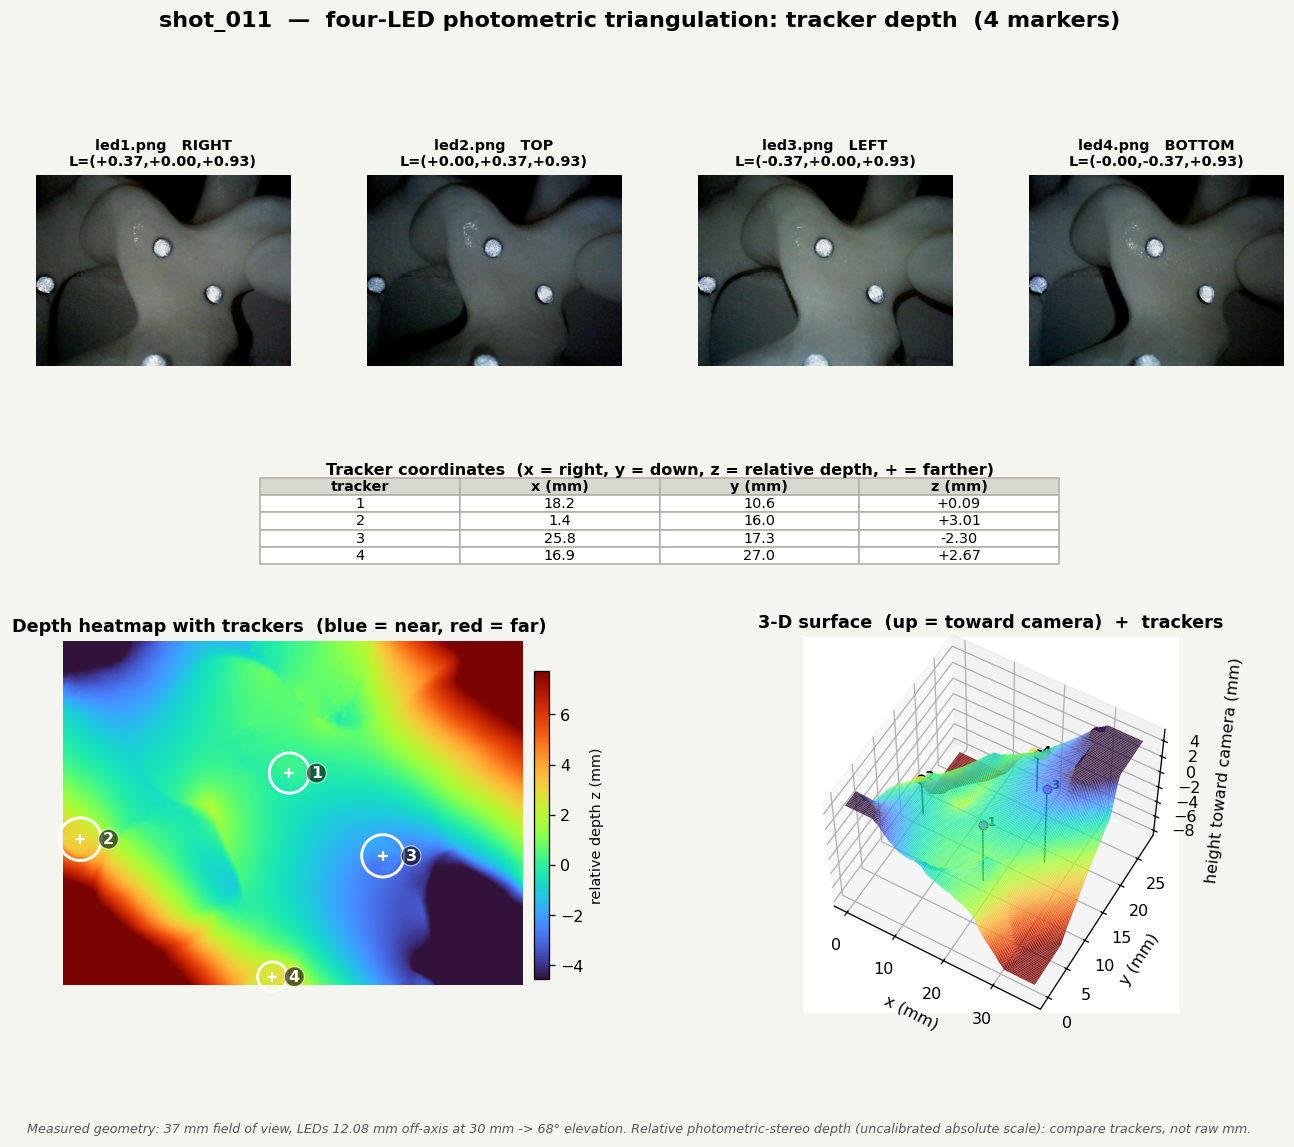
\includegraphics[width=0.92\textwidth]{../depth_outputs/marker_depth_slides/shot_011_marker_depth.png}
\caption{Per-session composite output for \texttt{shot\_011}. Top row: the four
single-emitter exposures with their light vectors. Middle: recovered fiducial
coordinates. Bottom left: the relative depth field with all four detected
fiducials circled and numbered. Bottom right: the same field as a 3-D surface
with a vertical stem at each fiducial. The depth field shown is the
\emph{far-field} baseline subsequently shown to be inverted
(Sec.~\ref{sec:inversion}); it is smooth and anatomically plausible, and nothing
in it signals the failure.}
\label{fig:slide}
\end{figure*}

\subsection{Far-field depth against CT: the inversion}\label{sec:inversion}
This is the paper's principal empirical result.

For the three CT-known fiducials, the P3P solution of Sec.~\ref{sec:p3p} --- the
branch placing fiducial~4 nearest --- gives lens distances of
\SI{33.5}{\milli\metre} (fiducial~4), \SI{50.9}{\milli\metre} (1) and
\SI{53.2}{\milli\metre} (3), spanning \SI{19.7}{\milli\metre}. Converted to
camera-frame depth relative to the fiducial-set median, the CT values span
\SI{20.7}{\milli\metre}. The far-field photometric depths for the same three
fiducials are $+0.087$, $-2.302$ and $+2.673$\,mm (Table~\ref{tab:inversion}).

\begin{table}[t]
\centering
\caption{Far-field photometric depth versus CT ground truth,
\texttt{shot\_011}. All values in millimetres.}
\label{tab:inversion}
\footnotesize
\begin{tabular}{@{}lrrrrr@{}}
\toprule
\textbf{Fid.} & $z_\mathrm{est}$ & \textbf{CT $z_\mathrm{rel}$} &
\textbf{CT dist.} & $z_\mathrm{corr}$ & \textbf{resid.} \\
\midrule
1 & $+0.087$ & $0.000$    & 50.9 & $-6.157$  & $-6.157$ \\
3 & $-2.302$ & $+0.719$   & 53.2 & $+3.920$  & $+3.201$ \\
4 & $+2.673$ & $-20.023$  & 33.5 & $-17.066$ & $+2.957$ \\
2 & $+3.011$ & ---        & ---  & $-18.492$ & --- \\
\bottomrule
\end{tabular}
\end{table}

\begin{figure*}[t]
\centering
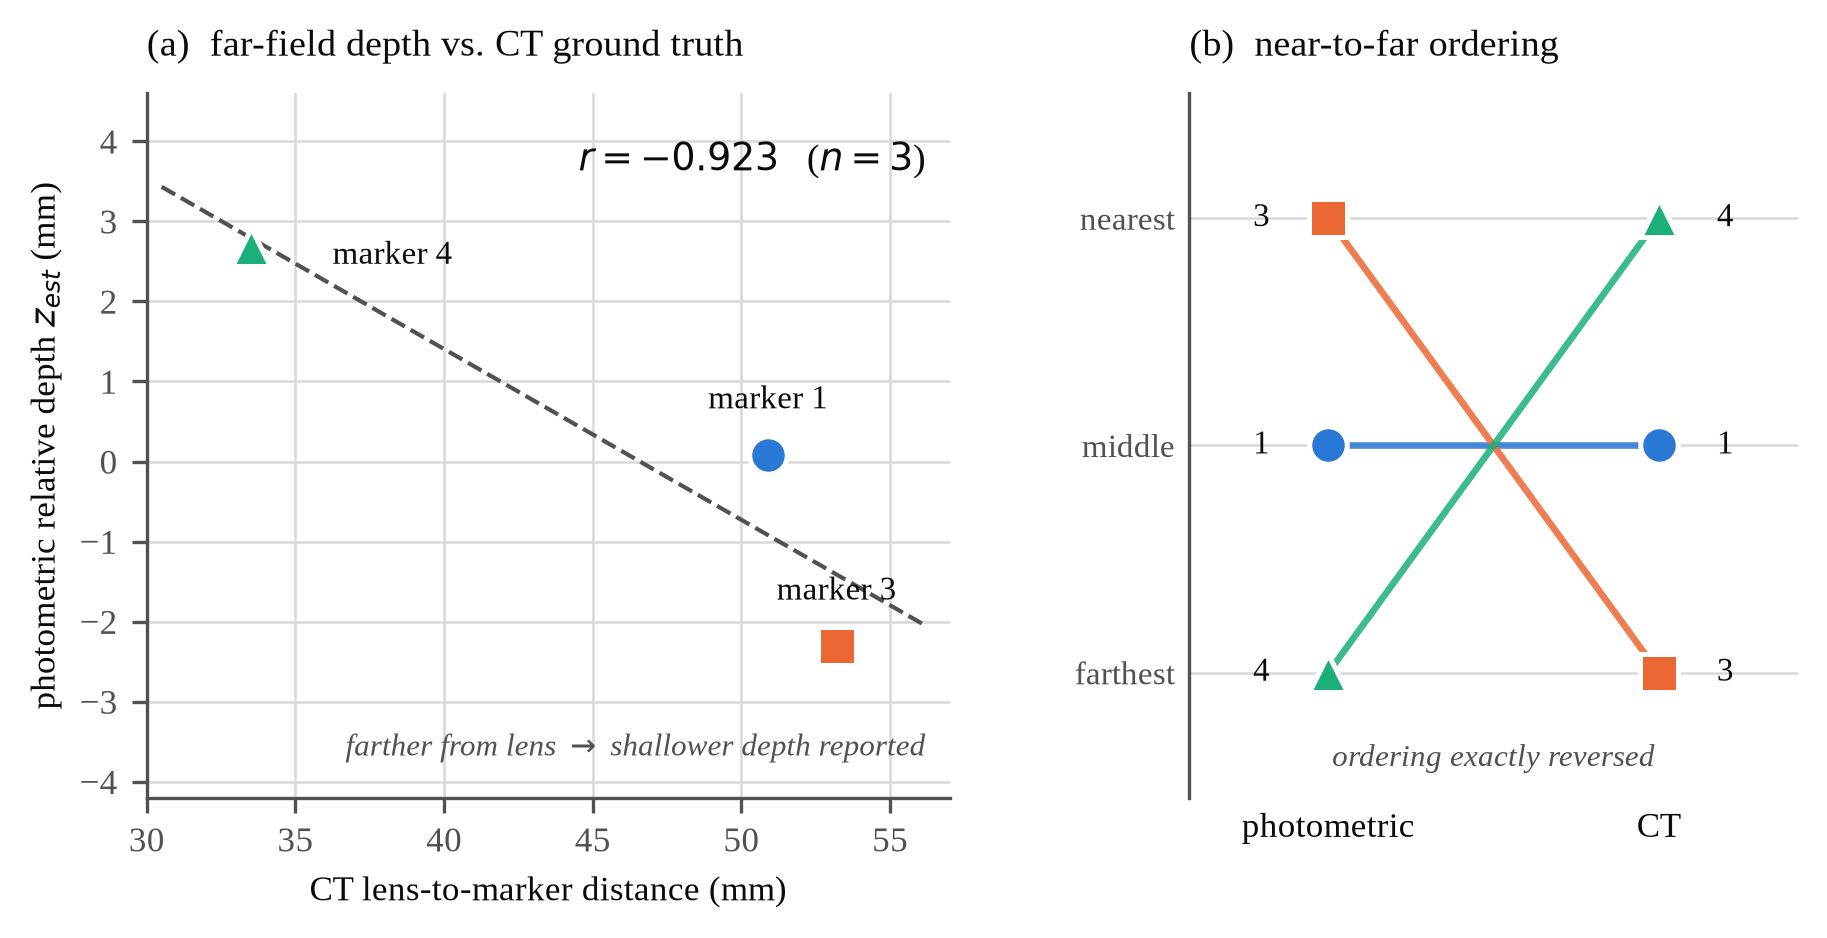
\includegraphics[width=0.88\textwidth]{fig2_inversion.png}
\caption{The depth inversion at \texttt{shot\_011}. (a) Far-field photometric
relative depth against CT-derived lens-to-fiducial distance, with the
least-squares trend (dashed). The relationship is negative: fiducials that CT
places \emph{farther} from the lens are assigned \emph{shallower} depth.
(b) Near-to-far ordering under each method. Fiducial~1 holds the middle position
while 3 and 4 exchange the extremes, reversing the sequence $(3,1,4)$ to
$(4,1,3)$. Identity is encoded by colour \emph{and} symbol so the figure survives
greyscale reproduction.}
\label{fig:inversion}
\end{figure*}

Three findings follow (Fig.~\ref{fig:inversion}).

\textbf{(i) The correlation is negative.} Pearson correlation between far-field
relative depth and CT lens-to-fiducial distance is $r = -0.923$; against
camera-frame CT depth it is $r=-0.891$. The depth channel varies inversely with
true distance.

\textbf{(ii) The ordering is reversed.} Ranked nearest to farthest, photometry
gives $(3,1,4)$ where CT gives $(4,1,3)$. This is not noise degrading a correct
ordering; it is a systematic sign inversion.

\textbf{(iii) Affine correction cannot rescue it.} Least-squares affine fitting
onto the CT control points returns
\begin{equation}
z_\mathrm{corr} = -4.218\, z_\mathrm{est} - 5.791 \ \ \text{mm},
\end{equation}
whose \emph{negative slope} states the inversion algebraically. Even permitting
the sign flip, the fit leaves \SI{4.36}{\milli\metre} RMS across a
\SI{20.7}{\milli\metre} true span --- about \SI{21}{\percent} of the measured
range. With two free parameters and three control points, this residual reflects
genuine lack of fit rather than an interpolation artifact.

The corrected map is retained as a diagnostic only: an affine rescale with slope
$-4.218$ amplifies the underlying far-field spatial bias roughly threefold while
merely re-seating the fiducial values.

This is the empirical case for near-light modelling. The failure is a predictable
consequence of $\eta = 0.40$ (Sec.~\ref{sec:whyfar}), not of implementation, and
it cannot be repaired downstream: the artifact is spatially varying, so a global
affine correction cannot remove it, and the tilt-plane alternative needs three
non-collinear control fiducials, which only one session provides --- and there it
interpolates exactly, yielding no residual information. The forward model must be
fixed instead.

\subsection{Lens-to-fiducial distances}
Eighteen distances were computed, of which three are CT-validated and fifteen
photometric and flagged unreliable. The CT-validated values are \num{50.9},
\num{53.2} and \SI{33.5}{\milli\metre}; these are trustworthy up to the
${\sim}1.5\times$ scale ambiguity of Sec.~\ref{sec:ambiguity}, which is
multiplicative and therefore affects neither their ordering nor their ratios.
The photometric values have mean \SI{48.6}{\milli\metre} and standard deviation
\SI{4.4}{\milli\metre}.

The apparent tightness of that distribution is \emph{not} evidence of accuracy.
Those values are constructed by adding a small relative depth (SD
\SI{2.25}{\milli\metre}) to a \emph{constant} \SI{46.0}{\milli\metre} anchor and
back-projecting, so their spread is largely inherited from the anchor by
construction --- and the component that does vary is the very quantity shown
above to be sign-inverted.

\begin{notebox}{Two defects in the anchor itself}
The implementation documents \SI{46.0}{\milli\metre} as the \emph{median} P3P
distance. It is not: the three CT-validated distances have median
\SI{50.92}{\milli\metre} and mean \SI{45.84}{\milli\metre}, so the constant
matches the mean, not the median. Its provenance is genuinely ambiguous ---
\SI{45.9}{\milli\metre} is also the working distance implied by the checkerboard
focal length --- and it must be settled and the label corrected, since fifteen of
the published rows depend on it. Separately, the anchor is a \emph{Euclidean}
distance statistic but is used as an \emph{axial} depth $Z$ before multiplication
by the ray norm, applying the obliquity factor twice: negligible
(\SI{0.59}{\percent}) for a near-axial fiducial but \SI{15.3}{\percent} for the
most off-axis one. Both are small against the declared unreliability of these
rows, but both are definite errors.
\end{notebox}

\subsection{A scale conflict no focal length resolves}\label{sec:scaleconflict}
Section~\ref{sec:ambiguity} reported the focal-length discrepancy as a
${\sim}1.53\times$ ambiguity. Cross-checking the pose solution against the bench
geometry reveals something stronger, and we report it because a reviewer holding
Table~\ref{tab:ct} and the fiducial pixel coordinates can reproduce it in a few
lines.

Feeding $f_x=\SI{519}{pixel}$ --- itself \emph{derived} from the premise
$d_\mathrm{work}=\SI{30}{\milli\metre}$ --- into the P3P solve returns a median
axial depth of \SI{50.62}{\milli\metre}, \num{1.69} times that premise. This is
not a focal-length ambiguity, because the P3P scale is fixed by the known metric
size of the CT triangle, which makes the \emph{implied} field width
$\Omega' = W Z/f_x$ almost independent of $f_x$ (Table~\ref{tab:fxsweep}).

\begin{table}[t]
\centering
\caption{Implied field width as a function of assumed focal length. The recovered
depth scales with $f_x$, so the implied field width is nearly invariant --- and
never approaches the measured \SI{37}{\milli\metre}.}
\label{tab:fxsweep}
\footnotesize
\begin{tabular}{@{}lrrrrr@{}}
\toprule
$f_x$ (px, at $W{=}640$) & 300 & 519 & 794 & 1000 & 2000 \\
\midrule
median $Z$ (mm)          & 28.6 & 50.6 & 75.3 & 93.9 & 184.6 \\
implied $\Omega'$ (mm)   & 61.1 & 62.4 & 60.7 & 60.1 & 59.1 \\
\bottomrule
\end{tabular}
\end{table}

Across $f_x$ from \SIrange{300}{2000}{pixel} the implied field width stays within
\SIrange{59.1}{62.8}{\milli\metre}, i.e. \numrange{1.60}{1.70} times the
\SI{37.0}{\milli\metre} bench figure, and a root search finds \emph{no} $f_x$ in
\SIrange{250}{1400}{pixel} at which $\Omega' = \SI{37}{\milli\metre}$. Neither
candidate focal length reconciles the two. The conflict is with the field-width
measurement, not with $f_x$.

The same tension appears independently in the fiducial geometry. The CT
pairwise separations are \SI{17.18}{}, \SI{27.57}{} and
\SI{26.20}{\milli\metre}; at the \SI{37}{\milli\metre} scale their ratios to the
projected separations are \numrange{1.67}{1.99}, which requires the fiducial
plane to be tilted \SI{53.8}{\degree} from the image plane. At the P3P-implied
scale the ratios fall to \numrange{1.09}{1.30}, a far more natural configuration.

\begin{todobox}{Unresolved --- two candidate explanations, and we cannot yet
distinguish them}
\textbf{(i) The \SI{37}{\milli\metre} field-width measurement is wrong} by a
factor near \num{1.7}. \textbf{(ii) The CT-to-detection correspondence is wrong.}
The detector assigns fiducial indices purely by image position (top-to-bottom,
then left-to-right); that ordering bears no necessary relation to the CT
numbering, yet the distance code assumes detection index $i$ equals CT fiducial
$i$. This assumption is nowhere verified.

Enumerating all \num{24} assignments of the three CT points to the four
detections, and keeping only those that place fiducial~4 nearest with all
distances physically possible, leaves eight candidates whose implied field widths
are \SIlist{44.2;44.4;45.5;46.8;47.0;47.1;58.7;62.4}{\milli\metre}. The
pipeline's own assignment is the \emph{worst} of the eight, and \textbf{none
reaches \SI{37}{\milli\metre}}. Permutations that would imply ${\sim}\SI{37}{
\milli\metre}$ each require either a fiducial at \SIrange{6.7}{7.8}{\milli\metre}
from the lens (impossible) or fiducial~4 to be farthest, contradicting the
confirmed physical ordering.

\textbf{Required:} re-measure the field width, and independently establish the
CT-to-detection correspondence --- then report the check either way. Until this
is settled, absolute distances should be quoted with the conflict stated, not
merely with the ${\sim}1.53\times$ focal ambiguity. See Appendix~\ref{app:open},
items~C2 and~C8.
\end{todobox}

Note that this conflict does \emph{not} weaken the inversion result of
Sec.~\ref{sec:inversion}: correlation and rank ordering are invariant under any
positive rescaling of the CT distances, and the ordering constraint used to
select the pose is unaffected.

\subsection{Calibration self-tests}\label{sec:selftest}
Both auxiliary modules ship self-tests on synthetic ground truth, runnable
without captured data. Both pass (Table~\ref{tab:selftest}).

\begin{table}[t]
\centering
\caption{Self-test results on synthetic ground truth.}
\label{tab:selftest}
\footnotesize
\begin{tabular}{@{}llr@{}}
\toprule
\textbf{Module} & \textbf{Stage} & \textbf{Result} \\
\midrule
correction & affine-$z$, 2 control pts & 0.015, 0.006, 0.008 mm \\
correction & tilt-plane, 3 control pts & 0.030, 0.046 mm \\
LED calib. & anisotropy, $\theta_{1/2}=\SI{60}{\degree}$ & $\mu = 1.0000$ \\
LED calib. & position (mirror ball) & \SI{0.00}{\milli\metre} \\
LED calib. & direction / intensity & \SI{0.090}{\degree} / \SI{0.01}{\percent} \\
\bottomrule
\end{tabular}
\end{table}

The passing affine-$z$ test does \emph{not} license the affine correction of
Sec.~\ref{sec:inversion}: it confirms the estimator recovers a scale-and-offset
distortion, whereas the real distortion is a spatially varying near-light bias
that this model is not designed to remove.

More importantly, we must report what these tests do \emph{not} establish,
because we tested that question directly by mutation rather than by inspection.

\begin{todobox}{The self-tests are not sound validation as currently written}
Each test renders a synthetic scene with the same forward model the solver
inverts, and generator and solver share the physical relations under test. We
verified the consequences by deliberately corrupting the code:

\begin{itemize}
\item \textbf{The emitter-position test cannot distinguish correct from
incorrect geometry.} Replacing $\sin\beta$ with $\tan\beta$ in the solver and
$\arcsin$ with $\arctan$ in the generator --- a fundamentally wrong tangent-cone
relation --- still passes, at \SI{3e-12}{\milli\metre}. Worse, running the
\emph{wrong} solver against a \emph{correct} generator passes the shipped
\SI{2.0}{\milli\metre} threshold on 10 of 12 seeds, including the seed actually
shipped. The true noise-free round-trip error is \SI{2.5e-12}{\milli\metre},
twelve orders of magnitude below the assertion: the threshold is not a tolerance
but a blindfold.
\item \textbf{The $\cos^4$ vignetting law and the $1/r^3$ falloff are
tautological.} Each appears in identical form in generator and solver and
cancels exactly; changing the exponent in both simultaneously leaves the reported
errors bit-identical.
\item \textbf{The linearization is never exercised.} The direction/intensity test
hard-codes $\mu=1$, where $(\cdot)^{1/\mu}$ is the identity and the change of
variable $\vecm_s = \Psi^{1/\mu}\vecn_s$ degenerates. (Independent sweeps at
$\mu \in \{0.51, 1, 2, 4.82\}$ do confirm exact recovery, so no bug is hiding
here --- but the shipped test provides no evidence of it.)
\item \textbf{Error propagation between stages is untested.} Stage~2 receives the
exact $\vecx_s$, so it never sees Stage~1's error. Injecting a realistic
\SI{0.5}{\milli\metre} error in $\vecx_s$ produces \SI{2.09}{\degree} mean
direction error and \SI{1.18}{\percent} intensity error --- the dominant
real-world term, and invisible to the test.
\end{itemize}

\textbf{Required before submission:} tighten the position tolerance to
${\sim}\SI{1e-9}{\milli\metre}$; generate silhouettes by solving the ray--sphere
tangency condition, which is algebraically independent of
$\sin\beta = R/\lVert\bm{C}\rVert$; add a noisy variant with a justified
tolerance; exercise $\mu\neq1$; and report Stage-1$\to$Stage-2 propagation. See
Appendix~\ref{app:open}, item~C6.
\end{todobox}

What the tests \emph{do} establish is that the linear algebra correctly inverts
the model as the authors understand it. That is worth reporting, but it is not
validation of the model's fidelity to the rig, and the paper must not claim
otherwise.

\subsection{Registration results}\label{sec:regresults}
\begin{todobox}{NO REGISTRATION RESULT EXISTS}
Every number in this subsection is invented scaffolding, present only so the
results section has the correct shape. Nothing here may be cited or circulated.

Registration was evaluated over \TODO{N} correspondences from \TODO{M} sessions.
The closed-form similarity solution returned scale \TODO{S.SSS}, with rotation,
translation and scale residuals reported separately. \textbf{TRE} at independent
targets: mean \TODO{T.TT}, median \TODO{T.TT}, SD \TODO{T.TT}, maximum
\TODO{T.TT}, \SI{95}{\percent}ile \TODO{T.TT} mm, reported per target rather than
pooled. \textbf{FRE} (diagnostic only): \TODO{F.FF} mm RMS --- reported for
completeness and \emph{not} an accuracy claim.

Sensitivity to the focal-length ambiguity must be reported as a paired analysis
at $f_x = \num{519}$ and \SI{794}{pixel}, since a $1.5\times$ intrinsic error
propagates directly into recovered scale and translation.
\end{todobox}

\section{Discussion}

\subsection{What the pipeline supports today}
The clearest outcome is a sharp, measured separation between reliable and
unreliable outputs. Fiducial localization is robust: \SI{78}{\percent} of
fiducials were confirmed under four independent illumination conditions, and the
three-signature acceptance logic with its dark-surround requirement separates
retroreflectors from glints on wet bone. The CT/P3P distances rest on independent
ground truth and a physically disambiguated pose. Both are suitable registration
inputs.

The far-field depth channel is not. It is sign-inverted against the only
available ground truth, and every quantity derived from it inherits that
inversion. These outputs are retained and labelled as unreliable in the data
files themselves, so the failure is documented rather than hidden.

We stress that this separation was possible \emph{only} because one session
carried CT ground truth. With no ground truth, the depth maps of
Fig.~\ref{fig:slide} are entirely plausible --- smooth, with anatomically
sensible relief of a few millimetres, and fiducials at sensible depths. Nothing
in the output signals that the ordering is reversed. This is a general hazard of
shading-based reconstruction and argues for including ground-truth control points
in at least one session of any such study as routine design.

\subsection{The corrective path and its cost}
The near-light solver and its calibration constitute a complete, implemented and
unit-validated path to physically correct depth. The remaining cost is not
development but \emph{data acquisition} --- a mirror ball and a matte white card,
one session's work. Separately, the $1.53\times$ focal-length discrepancy must be
resolved before any absolute metric claim; it is settled by imaging an object of
known size at a known distance.

\subsection{Implications for registration}
\TODO{EXPAND ONCE SEC.~\ref{sec:reg} IS WRITTEN.} The inversion constrains the
registration design directly, and favourably. Because the depth channel is
unusable, registration cannot depend on it --- but the fiducial pixel coordinates
and the CT/P3P geometry are sound, and correspondence-based registration on
fiducials uses exactly those. A fiducial-correspondence formulation is therefore
not merely convenient but the only one the current data supports, and it is the
more rigorous choice regardless: it yields a closed-form solution and a directly
measurable target error, rather than an iterative fit whose residual can be low
for reasons unrelated to correctness.

\section{Limitations}
\begin{enumerate}
\item The far-field depth channel is sign-inverted ($r=-0.923$), invalidating the
depth column for all sessions and the fifteen photometric distances.
\item Ground truth exists for one session and three fiducials ($n=3$). The
correlation and ordering findings are unambiguous at this $n$; the affine
residual is a weak estimate.
\item The ground truth's own uncertainty is unquantified.
\item Absolute scale is unresolved. Beyond the ${\sim}1.53\times$ focal-length
ambiguity, the pose solution implies a field width of
\SIrange{59}{63}{\milli\metre} for \emph{any} focal length, conflicting with the
\SI{37}{\milli\metre} bench measurement (Sec.~\ref{sec:scaleconflict}); either
that measurement or the CT-to-detection correspondence is wrong. The calibration
reprojection residual is also unrecorded.
\item The principal point is set to the image centre rather than its calibrated
value, a \SI{14.5}{pixel} vertical discrepancy worth
\SIrange{0.1}{0.7}{\milli\metre} on the reported distances.
\item The calibration self-tests share their forward model with the solvers and,
for emitter position, carry a tolerance loose enough to pass demonstrably wrong
geometry (Sec.~\ref{sec:selftest}). They validate implementation, not model
fidelity.
\item The near-light path has never been run on real data, pending calibration
captures.
\item Capture conditions --- ambient control, auto-exposure and white-balance
settings, saturation --- are undocumented.
\item Two fiducials rest on single-frame detections.
\item Raw captures are not committed, so the pipeline cannot be re-executed
end-to-end from the repository alone.
\item Software versions are unpinned, which additionally makes one solver
citation version-dependent (Appendix~\ref{app:open}, item~M5).
\item \TODO{REGISTRATION LIMITATIONS --- PENDING}
\end{enumerate}

\section{Conclusion}
We have presented a near-light photometric stereo pipeline for a four-LED ring
endoscope: the ring geometry and its offset and scale calibration, a calibrated
point-source forward model, a perspective log-depth solver, per-emitter
photometric calibration, retroreflective fiducial localization, and
fiducial-anchored transfer into the CT frame.

Measured against CT, the far-field approximation fails at this geometry not by a
scale factor but in sign: the recovered depth is anti-correlated with truth
($r=-0.923$) and reverses the ordering of all three CT-known fiducials, and no
affine correction recovers it. With an offset-to-working-distance ratio of
\num{0.40}, this is the predictable consequence of applying a distant-source
model to a near-light rig. The calibrated near-light formulation is the
corrective path; it is implemented and passes synthetic validation, and is
blocked only on one session of calibration captures.

Fiducial localization and CT/P3P distances are reliable and constitute the
registration inputs the pipeline can support today.
\TODO{FINAL REGISTRATION CONCLUSION --- PENDING}

\appendices
\section{Open Items}\label{app:open}
\footnotesize
\textbf{Registration (principal claim).}
\textbf{R1}~Decide and document the registration formulation; resolve its
relationship to the existing P3P pose.
\textbf{R2}~Acquire per-session CT fiducial coordinates for
\texttt{shot\_012}--\texttt{015}.
\textbf{R3}~Produce the result: scale, per-parameter residuals, TRE per target,
FRE as diagnostic.
\textbf{R4}~Define and execute a validation protocol with independent targets;
state repetition count.
\textbf{R5}~Write the fiducial-configuration subsection and justify the
configuration.
\textbf{R6}~Report sensitivity to the focal-length ambiguity at both $f_x$
values.
\textbf{R7}~Log and report the P3P candidate-pose count and filter survival.
\textbf{R8}~Quantify CT ground-truth uncertainty as the validation noise floor.

\textbf{Measurement and calibration.}
\textbf{C1}~Capture LED calibration targets (mirror ball ${\sim}10$ poses per
emitter; matte white card \numrange{3}{5} tilts); record $\theta_{1/2}$, the
Arduino Pro variant, LED part number and drive current.
\textbf{C2}~Resolve the $f_x$ ambiguity; record reprojection residual, pose count
and distortion coefficients.
\textbf{C3}~Run the near-light solver on real data and re-validate against CT.
\textbf{C4}~Re-derive lens-to-fiducial distances from near-light depth.
\textbf{C5}~Obtain CT ground truth for the remaining fiducial in
\texttt{shot\_011}.
\textbf{C6}~Repair the calibration self-tests: tighten the position tolerance to
${\sim}\SI{1e-9}{\milli\metre}$, generate silhouettes by tangency solving rather
than by the cone parameterisation the solver inverts, add a noisy variant,
exercise $\mu\neq1$, and report inter-stage error propagation. Drop shadowed
pixels in the direction/intensity fit instead of clamping, and report the
surviving fraction. Emit conditioning diagnostics for the silhouette fit and the
ray triangulation.
\textbf{C7}~Record the measured $E_R/E_B$ of the emitters on a neutral target,
and state the datasheet angle convention ($\theta_{1/2}$ versus
$2\theta_{1/2}$) alongside the recorded value.
\textbf{C8}~Resolve the field-width conflict of Sec.~\ref{sec:scaleconflict}:
re-measure the field width, and independently establish the CT-to-detection
fiducial correspondence rather than assuming index equality.
\textbf{C9}~Correct the intrinsics: use the calibrated principal point rather
than the image centre, and fix the anchor-constant label and the axial/Euclidean
double-count in the photometric distance path.

\textbf{Manuscript.}
\textbf{M1}~Authors, affiliations, funding, competing interests, ethics and
specimen provenance (naming the oversight or licensing body), consent, data and
code availability, author contributions, AI-tool disclosure.
\textbf{M2}~Verify every reference against the publisher record --- several
entries are currently unverified (Appendix~\ref{app:refs}).
\textbf{M3}~Specimen description and fiducial physical diameter.
\textbf{M4}~Figure preparation at journal resolution.
\textbf{M5}~Pin software versions --- required for correctness of the solver
citation, not only reproducibility.
\textbf{M6}~Select target journal and reformat; abstract structure, declaration
headings and word budgets differ, and several budgets are inclusive of references
and captions.

\section{Reference Verification Status}\label{app:refs}
\footnotesize
Reference metadata is a common source of published error, and entries drawn from
third-party bibliography files are frequently corrupt. Publisher sites were not
reachable from the build environment, so most entries below could not be
confirmed against a publisher record.

\textbf{Verified:} \cite{queau2018led} (confirmed against the corresponding
author's released code repository); \cite{ke2017} (confirmed as the algorithm
implemented by OpenCV \texttt{SOLVEPNP\_AP3P}, by direct inspection of the OpenCV
source and its bibliography; proceedings pagination unverified).

\textbf{Unverified --- must be checked before submission:}
\cite{fitzpatrick1998,fitzpatrick2009,shamir2009,west2001,woodham1980,frankot1988}.

\textbf{Version-dependent citation.} The neighbouring OpenCV flag
\texttt{SOLVEPNP\_P3P} maps to Gao \textit{et al.}~(2003) in OpenCV 4.5.5 but to
a different algorithm on current 4.x releases. Our code calls
\texttt{SOLVEPNP\_AP3P}; pin the version or the citation is unfalsifiable.

\begin{thebibliography}{9}
\footnotesize
\bibitem{queau2018led}
Y.~Qu\'eau, B.~Durix, T.~Wu, D.~Cremers, F.~Lauze, and J.-D.~Durou,
``LED-based photometric stereo: Modeling, calibration and numerical solution,''
\emph{J. Math. Imaging Vis.}, vol.~60, no.~3, pp.~313--340, 2018.

\bibitem{ke2017}
T.~Ke and S.~Roumeliotis, ``An efficient algebraic solution to the
perspective-three-point problem,'' in \emph{Proc. IEEE Conf. Computer Vision and
Pattern Recognition (CVPR)}, 2017.

\bibitem{fitzpatrick1998}
J.~M.~Fitzpatrick, J.~B.~West, and C.~R.~Maurer, Jr., ``Predicting error in
rigid-body point-based registration,'' \emph{IEEE Trans. Med. Imag.}, vol.~17,
pp.~694--702, 1998. \TODO{UNVERIFIED}

\bibitem{fitzpatrick2009}
J.~M.~Fitzpatrick, ``Fiducial registration error and target registration error
are uncorrelated,'' in \emph{Proc. SPIE}, vol.~7261, 2009. \TODO{UNVERIFIED}

\bibitem{shamir2009}
R.~R.~Shamir, L.~Joskowicz, S.~Spektor, and Y.~Shoshan, ``Localization and
registration accuracy in image guided neurosurgery: A clinical study,''
\emph{Int. J. Comput. Assist. Radiol. Surg.}, vol.~4, pp.~45--52, 2009.
\TODO{UNVERIFIED}

\bibitem{west2001}
J.~B.~West \emph{et al.}, ``Fiducial point placement and the accuracy of
point-based, rigid body registration,'' \emph{Neurosurgery}, vol.~48, no.~4,
pp.~810--816, 2001. \TODO{UNVERIFIED}

\bibitem{woodham1980}
R.~J.~Woodham, ``Photometric method for determining surface orientation from
multiple images,'' \emph{Opt. Eng.}, vol.~19, no.~1, pp.~139--144, 1980.
\TODO{UNVERIFIED}

\bibitem{frankot1988}
R.~T.~Frankot and R.~Chellappa, ``A method for enforcing integrability in shape
from shading algorithms,'' \emph{IEEE Trans. Pattern Anal. Mach. Intell.},
vol.~10, no.~4, pp.~439--451, 1988. \TODO{UNVERIFIED}
\end{thebibliography}

\end{document}
